\section{El Sistema de los Números Reales}

Todas las ecuaciones lineales de la forma $bx=a$ (con $a,b\in\mathbb{Z}$ y $b\neq 0$) tienen solución en el conjunto de los racionales $\mathbb{Q}$. Sin embargo, si la ecuación involucra potencias, esto no siempre ocurre.

Históricamente, la crisis de los números racionales surgió al intentar medir la diagonal de un cuadrado de lado 1. Según el Teorema de Pitágoras, dicha diagonal $x$ debe cumplir $x^2 = 1^2 + 1^2$, es decir, $x^2-2=0$. Se puede demostrar que \textbf{no existe} ningún número racional $\frac{p}{q}$ que, elevado al cuadrado, resulte en $2$.

\subsection{Números Irracionales ($\mathbb{I}$)}
Para resolver ecuaciones como $x^2=2$, necesitamos introducir nuevos números. Al intentar escribir la solución positiva ($x=\sqrt{2}$) en notación decimal, encontramos que su desarrollo es \textbf{infinito y NO periódico}:
\[ \sqrt{2} \approx 1,41421356\dots \]

Este tipo de números conforma el conjunto de los \textbf{Números Irracionales}, denotado usualmente como $\mathbb{I}$ (o $\mathbb{R} \setminus \mathbb{Q}$). Se caracterizan por tener una expansión decimal infinita sin ningún patrón repetitivo. Algunos ejemplos notables son:
\begin{itemize}
    \item El número Pi: $\pi \approx 3,14159\dots$ (relación entre la circunferencia y su diámetro).
    \item El número de Euler\footnote{Base de los logaritmos naturales.}: $e \approx 2,71828\dots$
    \item La razón áurea: $\phi = \frac{1+\sqrt{5}}{2} \approx 1,61803\dots$
\end{itemize}

\subsection{Números Reales ($\mathbb{R}$)}
Definimos el conjunto de los \textbf{Números Reales} como la unión disyunta de los conjuntos Racional e Irracional:
\[ \mathbb{R} = \mathbb{Q} \cup \mathbb{I} \]

Geométricamente, la importancia de $\mathbb{R}$ radica en la propiedad de \textbf{Completitud}: los números reales llenan por completo la recta numérica. A cada punto de la recta le corresponde un único número real, sin dejar ``huecos'', a diferencia de lo que ocurriría si solo usáramos racionales.

\begin{figure}[ht]
    \centering
    \caption{Recta Real $\mathbb{R}$ con ubicación aproximada}
    \label{fig:rectareal}
    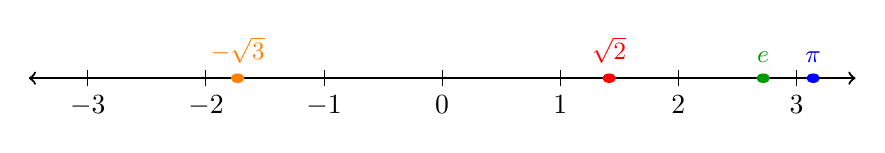
\begin{tikzpicture}[xscale=1.5]
        % Eje
        \draw[<->, thick] (-3.5,0) -- (3.5,0);
        % Ticks enteros
        \foreach \x in {-3,-2,-1,0,1,2,3}
            \draw (\x,0.1) -- (\x,-0.1) node[below] {$\x$};
        
        % Irracionales notables
        \draw[red, fill] (1.414,0) circle (1.5pt) node[above=2pt] {\small $\sqrt{2}$};
        \draw[blue, fill] (3.141,0) circle (1.5pt) node[above=2pt] {\small $\pi$};
        \draw[green!60!black, fill] (2.718,0) circle (1.5pt) node[above=2pt] {\small $e$};
        \draw[orange, fill] (-1.732,0) circle (1.5pt) node[above=2pt] {\small $-\sqrt{3}$};
    \end{tikzpicture}
\end{figure}

\subsection{Propiedad de Densidad}
Una propiedad fundamental, que comparten tanto $\mathbb{Q}$ como $\mathbb{R}$, es que son conjuntos \textbf{densos}. Esto significa que entre cualquier par de números distintos, siempre existe otro número (y, por ende, infinitos).

\begin{proposition}[Densidad de $\mathbb{R}$]
    Si $a,b\in\mathbb{R}$ con $a<b$, entonces existe un $c\in\mathbb{R}$ tal que $a<c<b$.
\end{proposition}

\begin{proof}
    Consideremos el punto medio $c=\dfrac{a+b}{2}$.
    Como $a<b$, sumando $a$ a ambos lados obtenemos:
    \[ 2a < a+b \implies a < \frac{a+b}{2} \]
    Análogamente, sumando $b$ a la desigualdad original:
    \[ a+b < 2b \implies \frac{a+b}{2} < b \]
    Por lo tanto, $a < c < b$.
\end{proof}

\subsection{Los Números Complejos ($\mathbb{C}$)}
Aunque $\mathbb{R}$ permite resolver innumerables problemas, existen ecuaciones algebraicas simples sin solución real, como $x^2+1=0$ (ya que el cuadrado de cualquier número real es positivo o cero).

Esto motiva la definición de la \textbf{unidad imaginaria} $i$, tal que $i^2 = -1$. A partir de ella se construye el conjunto de los \textbf{Números Complejos}:
\[ \mathbb{C} = \{ a+bi \mid a,b \in \mathbb{R} \} \]
Donde $a$ es la parte real y $b$ la parte imaginaria. Como todo real puede escribirse como $a+0i$, se concluye la jerarquía mostrada en la Figura \ref{fig:diagrama_complejos}: $\mathbb{N} \subset \mathbb{Z} \subset \mathbb{Q} \subset \mathbb{R} \subset \mathbb{C}$.

\begin{figure}[ht]
    \centering
    \caption{Jerarquía de los conjuntos numéricos}
    \label{fig:diagrama_complejos}
    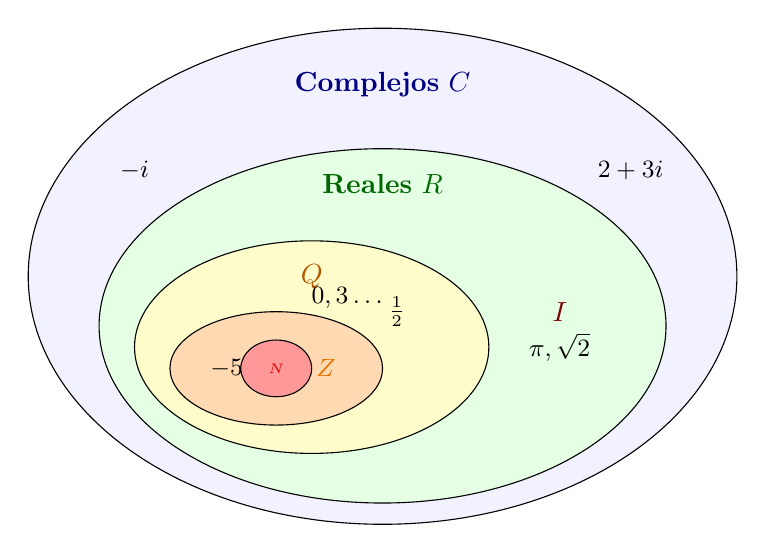
\begin{tikzpicture}[scale=0.9]
        % Definición de estilos para consistencia
        \tikzstyle{set} = [draw, ellipse, minimum width=2cm, thick]
        
        % C: Complejos (Elipse más grande)
        \draw[fill=blue!5] (0,0.5) ellipse (5cm and 3.5cm);
        \node[blue!50!black] at (0, 3.2) {\textbf{Complejos} $\mathbb{C}$};
        \node at (3.5, 2) {\small $2+3i$};
        \node at (-3.5, 2) {\small $-i$};

        % R: Reales
        \draw[fill=green!10] (0,-0.2) ellipse (4cm and 2.5cm);
        \node[green!40!black] at (0, 1.8) {\textbf{Reales} $\mathbb{R}$};
        
        % I: Irracionales (En R pero fuera de Q)
        \node[red!50!black] at (2.5, 0) {$\mathbb{I}$};
        \node at (2.5, -0.5) {\small $\pi, \sqrt{2}$};

        % Q: Racionales
        \draw[fill=yellow!20] (-1,-0.5) ellipse (2.5cm and 1.5cm);
        \node[orange!70!black] at (-1, 0.5) {$\mathbb{Q}$};
        \node at (0.2, 0) {\small $\frac{1}{2}$};
        \node at (-0.5, 0.2) {\small $0,3\dots$};

        % Z: Enteros
        \draw[fill=orange!30] (-1.5,-0.8) ellipse (1.5cm and 0.8cm);
        \node[orange!90!black] at (-0.8, -0.8) {\small $\mathbb{Z}$};
        \node at (-2.2, -0.8) {\small $-5$};

        % N: Naturales
        \draw[fill=red!40] (-1.5,-0.8) ellipse (0.5cm and 0.4cm);
        \node[red!90!black] at (-1.5, -0.8) {\tiny $\mathbb{N}$};
    \end{tikzpicture}
\end{figure}

\section*{Ejercicios Propuestos }

\begin{enumerate}
    \item \textbf{Irracionalidad entre Racionales:}
    Encuentre un número irracional que esté estrictamente entre $\frac{1}{2}$ y $\frac{1}{3}$. 
    \textit{Sugerencia: Intente modificar el promedio de ambos números dividiéndolo por un factor irracional pequeño o sumando un irracional muy pequeño.}

    \item \textbf{Refutación de Patrones:}
    Un estudiante afirma que ``la raíz cuadrada de cualquier número primo siempre es irracional''. ¿Es esto verdadero? Intente demostrarlo o buscar un contraejemplo.

    \item \textbf{Densidad y Aproximación:}
    Sabemos que $\pi$ es irracional. Sin embargo, para efectos prácticos usamos $3,1416$. Encuentre dos números racionales $a$ y $b$ (con denominador menor a 10) tales que $a < \pi < b$.

    \item \textbf{Potencias de la unidad imaginaria:}
    Calcule las potencias $i^1, i^2, i^3, i^4, i^5$. ¿Observa algún patrón cíclico? Basado en esto, calcule cuánto vale $i^{100}$.
\end{enumerate}
